\documentclass[BIT, graphvis, a4paper]{usydthesis}

\usepackage[final]{pdfpages} 
\usepackage[toc,page]{appendix}
\usepackage[utf8]{inputenc}
\usepackage{amsfonts}
\usepackage{amsmath}
\usepackage{amssymb}
\usepackage{caption} 
\usepackage{color} 
\usepackage{chngpage}
\usepackage{float}
\usepackage{framed}
\usepackage{fullpage}
\usepackage{graphicx}
\usepackage{hyperref} 
\usepackage{listings} 
\usepackage{subcaption} 
\usepackage[
    backend=biber,
    natbib=true,
	style=numeric,
    url=true, 
    doi=true,
    eprint=false
]{biblatex}
\usepackage{tabularx} 
\usepackage{tabu} 
\usepackage{tikz} 
\usepackage{url}
\usepackage{wrapfig} 

\addbibresource{bibliography.bib}
\newcommand{\littitle}[1]{
\subsection{\citetitle{#1}~\textcite{#1}}
}
 

\usetikzlibrary{arrows}
\usetikzlibrary{shapes,snakes}
\usetikzlibrary{positioning,calc}
\DeclareUnicodeCharacter{00A0}{ }
\newcommand*\rot{\rotatebox{90}}
\makeatletter
\newcommand{\@chapapp}{\relax}%
\makeatother
\graphicspath{ {images/} }
\setlength{\parskip}{\baselineskip}%
\setlength{\parindent}{0pt}%
% graph settings
\definecolor{nodeyellow}{RGB}{255,252,135}
\definecolor{nodeblue}{RGB}{179,255,255}
\tikzset{
	every node/.style={font=\sffamily\scriptsize}
}
\tikzset{
	group/.style={font=\sffamily,fill=nodeblue}
}
\tikzset{
	->,>=stealth',shorten >=1pt,auto,node distance=3cm,
	thick,main node/.style={ellipse,fill=nodeyellow,draw,font=\sffamily\normalsize}
}

% give captions a bit of space.
\captionsetup[sub]{margin=5pt, skip=10pt}

% listings style for prov code
\lstdefinestyle{provn}{
	breaklines=true,
	showstringspaces=false,
	basicstyle=\footnotesize\ttfamily,
}
\lstdefinestyle{basic}{
	breaklines=true,
	showstringspaces=false,
	basicstyle=\footnotesize\ttfamily,
	keywordstyle=\color{black},
	commentstyle=\color{black},
	stringstyle=\color{black},
}


\title{Clustering Provenance}

\begin{document}
\author{Linus Karsai}

\pagenumbering{roman}
\maketitle
\tableofcontents
% reset the page numbering and change to arabic numbers
\newpage\setcounter{page}{1}\pagenumbering{arabic}

\chapter{Abstract}

As digital objects become increasingly important in people's lives, people may need to understand the 
\emph{provenance}, or lineage and history, of an important digital object,
to understand how  it was produced.
This is particularly important for objects created from large, multi-source collections of personal data.
As the metadata  describing provenance, Provenance Data, is commonly represented as a labelled directed acyclic graph,
the challenge is to create effective interfaces onto such graphs
so that people can understand the provenance of key digital objects.
This unsolved problem is especially challenging for the case of novice and intermittent users and
complex provenance graphs.

We tackle this by creating an interface based on a \emph{clustering} approach.
This was designed to enable users to view provenance graphs,
and to simplify complex graphs by combining several nodes.

Our core contribution is the design of an interface that supports clustering
and its analytic evaluation in terms of desirable properties of visualisation interfaces.
 % abstract of thesis

\chapter{Introduction}

Provenance as a concept has been around for a long time. It originally comes from the Latin word \textit{provenio}, meaning ``to come forth''. It's primary use is in the field of antiques where provenance is used to identify the authenticity and quality of something. For anyone with a backgruond in databases this term may also be fimilair as linking tuples in a query output to the reasons they exist.

In this paper the provenance we refer to is that of \textit{digital provenance}. It is a type of metadata representing the lineage of an object. Naively it can be compared to the information stored in revision history systems like that used in google docs\footnote{Google docs: \url{https://docs.google.com}} or version control
% TODO: git and mercurial links
systems such as git\footnote{GIT\: \url{}} or mercurial. These systems are usually limited to storing revisions as well as authorship. However extends beyond this by making it posible to store and ultimately trace what other things and activities led to a digital object been in its current state.

Provenance has the potential for usefulness in many different fields. The foremost and focus of this paper is the field of personal data management, allowing users to understand how their data is used. Often when a user chooses to share their personal data it is aggregated, anonymised or passed through any number of functions. By exploring provenance users have the ability to understand exactly how much and in what state their personal data is used.

An example to illistrate this point. Alice has a report that describes her current fitness level as well as outlining possible improvements. Viewing the provenance of
% TODO: Fitbit and Withings footnotes
this report shows which sources have been used (e.g. Fit-Bit data to track steps, Withings scale to track weight) and what processes analysed them. In this case it could show that Alice's fitness report was generated using step data from her FitBit data, passed through a summarisation process that summarises 15 minute interval data into daily steps. This shows tracing of lineage backwards in time, it is also possible to trace information forward, possibly in the case of errors in data. Alice remembers that she lent her FitBit to a friend to try for a week, causing errors in her data. Provenance would allow tracing of the errenous information forward to see what other processes and entities it effected and would need to be corrected.

Provenance is also potentially useful in any field where the lineage of an object needs to be stored. This could be extended to digital records of antiques or artwork. This would also be useful in data warehouse systems where information about data transformations as well as origin are stored. There is also research into storing provenance in
% TODO: reference to block chains
block-chains or similar systems to prevent medling of historical data where it to be used in high risk systems such as banks or accounting systems.

Early provenance systems stored provenance information in a variety of different flat
% TODO: prov reference
file formats. Since 2013, the PROV specification has provided a generic model for storing provenance with a number of serialisations (PROV-N, XML, JSON and RDF). PROV identifies provenance elements as three main concepts:

\begin{itemize}
	\item Entities: Physical, digital, conceptual objects
	\item Activities: Elements that cause an entity to come into existence
	\item Agents: Someone or something that can be assigned responsibility for an activity taking place.
\end{itemize}

The industry standard for representing these concepts is on an acyclic graph. An example of this with each of the three main concepts can be see in Figure~\ref{fig:key-concepts}.

\begin{wrapfigure}{r}{0.5\textwidth}
	\centering
	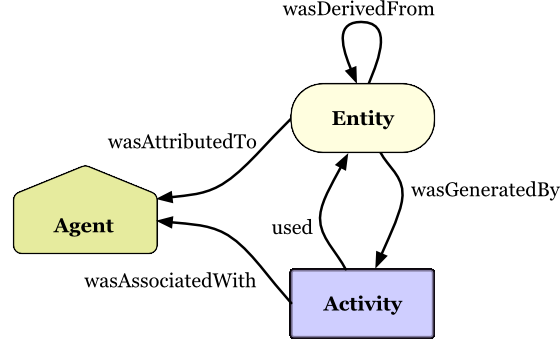
\includegraphics[width=\linewidth]{key-concepts}
	\caption{Key Concepts and relationships from the PROV standard displayed in a labelled acyclic graph.}
	\label{fig:key-concepts}
\end{wrapfigure}

Provenance can be stored in a variety of different granularity's and levels. The main three levels or provenance are system-level, application-level and network level. System level provenance is the lowest level and will often capture operating system activities such as which application ran at what to point to affect a piece of data. Application level provenance is limited to a single application, and will often capture information directly related to the user using that application. Network provenance captures information via network switches and stores lineage originating from multiple machines. These three levels are quire broad and do not cover all use cases but they do give a good point for starting discussion and comparing provenance capture tools. Provenance is also captured at different levels of granularity. Using the example of Alice as above, a system may capture information about her step data at the smallest granularity: how many steps every 15 minutes, or it may store the information at a larger granularity: aggregating step data daily.

As you can see in Figure~\ref{fig:key-concepts} provenance graphs are most often represented as directed acyclic graphs
% TODO: Novel provenance representation citing
although there has been some other novel approaches. The main problem we discuss is  provenance can become incredibly large, particularly in the case of OS level recording as it is usually at a low granularity so a lot of data is been recorded in a small time. Because provenance is inherently historical it is forever growing in size (as of yet there's no standard for going back and ``compressing'' history,) this means even  provenance captured as a high granularity will monotomiously grow and can become a graph with thousands or millions of nodes. This quickly becomes a
% TODO: usability studies chapter cite
usability problem as users can't visually digest such large graphs (results for usability studies in section x show that users are even put off by graphs with as little as 30 nodes).

What we describe in this paper is a process of simplifying graphs by clustering nodes into single composite nodes. A part from simplifying the graph and presenting less objects on screen, this also allows users to control what information is seen by other people or highlight particular concepts as seen in section x.
 % intro to pro etc.

\section{Related work}

\subsection{Provenance Overview}
\label{sec:provenance_overview}

As mentioned above, provenance is historically used in the field of antiques as a guide to authenticity of quality. In this thesis we focus on the more modern concept of digital provenance, a metadata that stores the lienage of a file. Only recently defined, below are two papers outlining the requirements and definition of digital provenance.

\relatedwork{Carata2014}
\label{sub:a_primer_on_provenance}

Published in the \textit{Communications of the ACM} magazine, this article gives an in depth introduction to digital provenance. It presents current research in the field from a practical perspective and talks at length about their possible use cases as well as issues obtaining, using and securing provenance.

This paper does an impressive job of laying out the fundamentals of digital provenance, as well as identifying current research efforts and areas of improvement. It also describes the language and terminology used by the provenance community when discussing different features of provenance, such as the concepts of \textit{granularity} and \textit{layering} when collecting provenance.

\relatedwork{Groth2012}
\label{sub:requirements_for_provenance_on_the_web}

This paper from \textit{The International Journal of Digital Curation} synthesizes three main categories that can be used to assess the adequacy of different online provenance systems. It splits these categories into multiple dimensions for finer grained analysis.

The three main categories this paper uses as a base for assessing provenance systems is: content (the data itself and information stored in it), management (different ways of collecting and storing the data) and use (different ways of using the data, visualisation etc.). Each of these categories is then divided into a multitude of related dimensions. For example the \textit{Content} category includes versioning (records of changes written to artefacts over time) and attribution (sources that contributed to making an artefact) as dimensions. The papers support their claims for the requirements of these dimensions by describing them in relation to three scenarios. The scenarios are well picked in order to mirror real world applications.

This paper outlines a range of dimensions that can by used in order to assess an interface. In terms of HCI these can be used as the base for tasks to test on users as well as suggesting features that may be useful in my application. For example, one of the dimensions for \textit{Use} is \textit{Imperfections}, suggesting that I need to take into account that erroneous/imperfect provenance data may exists when creating my interface.

\subsection{Provenance Acquisition}
\label{sec:provenance_acquisition}

Provenance can be acquired in a variety of ways. A common goal in the literature is to collect provenance automatically and transparently in order to reduce cognitive load on users as well as reducing erroneous or false data. The papers below discuss the collection of provenance across two different layers: operating system level and application level, both with their advantages and disadvantages.

\subsubsection{OS level provenance acquisition}
\label{sub:os_level_provenance_acquisition}

OS level provenance acquisition stores the calls between different processes and files. It has the advantage of clearly showing what applications rely on which resources and can be used via a custom kernel to log provenance on a computer without requiring any changes to the users applications.
However because of its intrinsic need to treat processes as ``black boxes'' it can also trigger false positives when graphing lineage. For example a process may invoke the use of multiple libraries however it is arguable as to whether they're all relevant in terms of provenance.

\relatedwork{Muniswamy2006}

Published in 2006, the PASS paper is often cited in related literature as a prime example of OS level provenance collection. This paper discusses the advantages of having provenance information maintained by the storage system as well as presenting a PASS implementation with analysis of its performance costs.

In most implementations provenance is stored in a standalone database systems or flat files. This paper argues that provenance should be maintained by the storage system since it is the storage system that manages existing metadata for files. This allows tighter coupling between data and provenance as well as allowing the transparent collection and management of provenance information. The paper lists a set of requirements for a PASS system as well as their own implementation. They benchmarked their implementation on a 500Mhz Pentium 3 computer with 768MB of RAM. The two primary benchmarks used are small and large file microbenchmarks. In the case of the small file benchmark the overhead associated with creating and writing files was as much as 200\%, however its noted that the absolute numbers are still quite small and that this benchmark in particular is quite challenging to PASS. Results from the large file benchmark where better with a time overhead of no more than \%10-\%20.  It seems more reasonable that real users will only encounter overheads of the latter in daily use. Overall the PASS system provides extra functionality not currently available in other systems with only a moderate overhead. It is also important to note that the systems used for these benchmarks are a lot less powerful that what average users use today.

\subsubsection{Application level provenance acquisition}
\label{sub:application_level_provenance_acquisition}

Application level provenance acquisition has the advantage of creating more relevant relationships between different entities. However it suffers from the overhead required to implement effective capturing and in a lot of cases onus on the user to annotate their actions. Most of the papers below discuss a system that requires developers to somehow modify (usually marginally) their application in order to correctly collect provenance.

\relatedwork{Guo2012}

Authored by Margo Seltzer (one of the top contributors of the field\cite{Macko2012,Seltzer2011,Borkin2013,Muniswamy-Reddy2010,Braun2008},) and Philip J. Guo, this paper presents one of the many ways to collect provenance on a computer. It focuses primarily on research relate provenance and its application in respect to \textit{lab notebooks}.

The application presented in this paper, Burrito, consists of two parts: an extensible platform that automatically captures provenance as well as a set of applications that allow annotations and querying of that data. Stored in a local MongoDB, provenance is captured though GUI window interactions, OS-level capture (like PASS\cite{Muniswamy2006}) and integration with a versioning filesystem. On top of this is a series of plugins that allow provenance to be captured by the following applications: microphone, xpad, Firebox, Chrome, Vim, Bash, Python and the clipboard. Burrito then provides four applications that allow interaction with the provenance data. An activity feed that sits on the users desktop, presenting provenance events chronologically and allowing annotation of events as they happen. A computation context viewer that allows exploration of a files changes and how they impacted output. An activity context viewer that shows what was been read and written at the time of an activity. Finally they also provide a Lab Notebook generator that creates a HTML file summarising the users activities. Over a month this system accumulates approximately 2GB of data and although no benchmarks are reported it is stated to have minimal overhead.

This paper is interesting as it brings provenance to the forefront of the users mind. The goal been that they are constantly annotating and referencing past provenance activities during the length of a project. It also has the added advantage of having images and other program output inline the visualisations.

\relatedwork{Macko2012}

Written in 2012 the authors of this paper Macko and Seltzer are both heavy contributors of the provenance field. Whilst most of the other provenance frameworks mentioned in this review are limited to a particular workflow or language, Macko and Seltzer argue that the real world is a lot more heterogeneous and to accommodate for this they argue the need for a general-purpose provenance library.

This paper presents the Core Provenance Library (CPL) a C++ application that allows the integration of provenance storage into any application. It supports bindings for C, Java and perl as well as a command a line tool for creating shell scripts. The provenance is stored on a database system of your choice through two drivers; these where tested to work for MySQL, PostgreSQl and 4store. The main disadvantage of this framework is that it is the onus of the developers to implement calls to the provenance framework in their application. Multiple features are implemented in order to allow easier integrating such as automatically taking care of persistent storage, cycle detection and resolution, as well as supporting query visualisation through map orbiter~\cite{Seltzer2011}. However developers/project managers need to take into consideration integration when developing an application.

This library provides hope for a standardised way of capturing provenance information. However as mentioned above it is up to developers to correctly integrate it and there's an intrinsic trust that correct and truthful provenance will be recorded. Disappointingly the \href{https://code.google.com/p/core-provenance-library/}{google code repository} hasn't been updated since 2012 and no replacement github repository has been created in light of the shutdown of Google code, suggesting that the project is no longer maintained.

\relatedwork{Allen2010}

This paper describes the ability to compose multiple provenance-unaware services in an ``open world'' system and collect provenance information about their execution. It presents a provenance collection application that sits upon the enterprise service bus (ESB) in order to log provenance information from communicating applications.

This paper advocates for a provenance collection solution that doesn't require system-invasive strategies such as custom kernels or modified applications. It argues that in order to be useful in the ``open world'' provenance capturing tools must fulfil the following tasks, capturing provenance:
\begin{itemize}
  \item across multiple systems with no assumption of control.
  \item from legacy systems
  \item at the level of application interaction, \textit{not} foundational technology stack.
\end{itemize}

In order to evaluate their ESB MULE Capturing Agent (MCA) they tested it upon two different workloads: Loan Borker (a standard MULE test scenario) and CoTLooper (a scenario that uses cursor on target messages). The average time to log provenance within MULE over time decreased as the more provenance nodes where created eventually evening out around $1 \times 10^8ns$. However if message reflection (a method for examining runtime behaviour of applications in the Java VM) was required to gather data from the payload of the message then message capture time can be greatly increased. Whilst these metrics are useful in identifying the overhead of using an ESB to capture provenance information from communicating applications (in this case minimal), itis arguable that the provenance information would suffer from problems similar to OS level capturing systems, creating false positive edges in the graph.

This paper is highly cited in the provenance community. It shows one of the many \textit{layers} of provenance that can be recorded and is one of the few systems that records provenance across multiple machines. 

\subsection{Provenance Storage}
\label{sec:provenance_storage}

Once provenance has been captured by one of the methods mentioned above, it has to be stored somehow. In a lot of early papers the provenance was stored in different proprietary flat file formats. Since then a standard has been created by the W3C, as well as research into how provenance can be stored on the cloud.

\relatedwork{primer2013}

This online document is an initiative by W3C to create a standard as by which to discuss and store digital provenance. This paper is part of a series of documents outlining different aspects of the PROV standard, in particular it is a primer on the fundamental PROV concepts.

This document outlines the three mains concepts illustrated in Figure~\ref{fig:key-concepts}, as well as different serialisations in languages such as XML, JSON and PROV-N. Each of the concepts are briefly described as:
\begin{itemize}
	\item Entities: Physical, digital, conceptual objects
	\item Activities: Elements that cause an entity to come into existence
	\item Agents: Someone or something that can be assigned responsibility for an actity taking place.  
\end{itemize}

\begin{figure}[h]
	\centering
	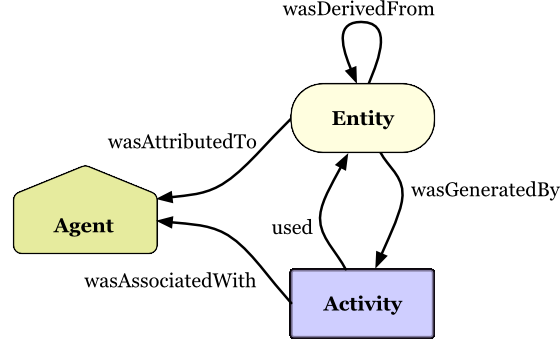
\includegraphics[width=0.5\linewidth]{key-concepts}
	\caption{Key concepts and relationships from the PROV standard displayed in a labelled acyclic graph.}
	\label{fig:key-concepts}
\end{figure}

I used the standards defined in this paper as the oracle definition for provenance in my designs. My prototype was built so that it can read provenance files in the PROV-N format.

\relatedwork{Muniswamy-Reddy2010}

This paper presents the following problem: although cloud data and provenance both exist, they are not usually used in conjunction because it is difficult to store both in the same location. Traditionally if data is stored in a database, the related provenance information is then stored somewhere else. To mitigate this they present 3 different methods for maintaining data and provenance in current cloud stores.

This paper's contribution is three protocols (using off the shelf software,) each satisfying a different number of properties crucial for provenance systems: provenance data coupling, multi-object casual ordering, data-independent persistence and efficient querying. Each of the systems work with minimal overhead and surprisingly the protocol that fulfils all four of the afore mentioned properties runs as well if not better than the other protocols. The benchmarks used on each of the protocols where varying in their workloads, ranging from CSV backup simulations to workloads representing scientific computation. There is a diverse selection of workloads that simulate scenarios that provenance would most likely be used in.

This creates an avanue of further research. Currently my prototype interface only reads locally stored flat provenance files. In the future it would be useful to expand this to provenance stored on the cloud as well.

\subsection{Provenance Security}
\label{sec:provenance_security}

Once provenance is captured and stored the issue of securing it is paramount. Simple per-attribute access permissions are ineffective for provenance entities because so much information can be gathered from relationships. It is alos worth considernig how to secure the data in such a way that history can't be ``re-written''. The below papers discuss this problem in greater detail.

\relatedwork{Braun2008}

A discussion paper from 2008, Margo, Uri and Avraham focus on the issue of properly securing the access rights of provenance data. It frames the problem and identifies issues requiring further research.

This paper aims to start discussion and highlight the importance of considering provenance security during the implementation and development of an application. It proves that provenance cannot be secured in the same way as traditional data because of its ability to provide information through relations as well as the artefacts themselves, arguing instead that provenance needs its own security model. The paper suggests that there is three main aspects of provenance that needs to be secured, each in their own way: the \textit{node data}, the \textit{relationships} between nodes and the \textit{attributes} related to nodes or relationships. It gives concrete examples of why each of these aspects need to be protected and why regular access control methods aren't satisfactory.

This piece is though provoking in the issues it outlines related to securing provenance. It raises the question of how to present partial graphs caused by users with limited permissions. A problem also worth considering in future work is that of how to present to a moderator which bits of a graph are accesible by who.

\relatedwork{Cheney2011}

A common theme among papers regarding provenance systems is that they agree that provenance is an open and unsolved issue. This paper from the University of Edinburgh outlines a formal model for provenance, formalization of security fundamentals \textit{disclosure} and \textit{obfuscation} and exploration of its implications in various domains.

This paper identifies five main classes of provenance policies: availability, confidentiality, integrity, reverse-engineering and explanation. They go on to describe a high level security framework focusing on the availability (ensuring information about input is available to users) and confidentiality (ensuring that confidential information is never disclosed to a user) of provenance data. This framework is general enough to not be specific to any one system, meaning its rules and obvservations can be applied to any system. The paper provides support to its claims through detailed mathematical proofs. It also provides three instances of how the provenance security framework can be used to create provenance policies.

Unfortunately this paper provides limited benefit to my project because its focus on security is abstract enough to be most useful to researchers designing provenance security systems. However it provides understanding of the security issues involved as well as ideas of how security will be implemented. 

\relatedwork{Hasan2009}

This paper is often referenced because of it work in creating \textit{Sprov}, a secure provenance storage method. 

The author's main contribution from this paper is \textit{Sprov}, a prototype of the secure provenance primitives, implemented as wrapper functions for the standard I/O library in C. They use a chain encryption method in order to accomplish their primary security goal: stopping undetected rewrites of history. In order to evaluate the Sprov library it was run through a number of benchmarks that simulate different deployment settings. They tested two different configurations for chain storage, both recording straight to disk and also storing on RAM with a chrom daemon periodically flushing the chain to disk. Postmart benchmark was used with a dataset containing 20,000 files ranging in size from 8KB to 64KB. Different write loads where tested all the way from 0-100\%. In its worse case scenario of 100\% writes, Sprov had an overhead of 25\% using disk storage and 11\% using RAM. Small and large file microbenchmarks was used to measure the overhead as a percentage of file size. Interestingly smaller files had a larger overhead, this is thought to be attributed to disk caching (similar results have been found by other provenance benchmarks).

This paper shows one of the many ways provenance data can be used and recorded. Its relevancy to my project is in understanding how provenance will be stored and protected as well as issues that arise in a user interface only showing partial data.

\subsection{Provenance Display}
\label{sec:provenance_display}

Lastly we come to the field of thesis. How to display provenance. As mentioned previously, provenance never reduces in size, it is forever expanding and been added to. Issues quickly arrise when trying to present such vast amounts of information. The primary issue been that users can't process such large graphs effectively.

\subsubsection{Visualisation fundamentals}
\label{sub:visualisation_fundamentals}

There's a series of fundamentals that have been tried and tested in the field of visualisation as important rules to follow when developing visualisation tools. Ben Shneiderman discusses fundamental tasks that should be accomplished by visualisation exploration software in order to be effective. A HCI paper then presents how non-technical users view provenance information.

\relatedwork{Shneiderman1996}

Published in 1996 this paper is seen as one of the core papers cited when discussing complex visualisation software. It recommends seven properties that should be implemented by an advanced graphical user interface: overview, zoom, filter, details-on-demand, relate, history and extract. It distils these tasks into what's known as the Visualisation Information Seeking Mantra:

\textit{Overview first, zoom and filter, then details-on-demand}\\
\textit{Overview first, zoom and filter, then details-on-demand}\\
\textit{Overview first, zoom and filter, then details-on-demand}\\
\textit{etc.}

Each of these tasks is explained in great detail with arguments as to why they are necessary. It also provides examples of how different applications have implemented certain tasks, providing an array of examples to research in regard to my project.

I used this paper as a primary starting point when creating my prototype. It was effective as a means of outlining the scope of my application, defining what features where and where not importand.

\relatedwork{Bachour2015}

A Human Centred Technology research project, this paper focuses on collecting feedback from non-expert uses on their understanding of provenance. Through the medium of an online game they explore how well users understand the W3 prov standard\cite{primer2013} and its related artifacts as well as their general opinions and beliefs on provenance data.

The main contributions taken from this paper involved the feedback users gave on the representation of provenance information: one example I found particularly interesting is that a lot of users found the directional arrows confusing. The PROV standard is historical, so directional arrows between nodes are used to represent that something came from something else, however most users found this counter-intuitive and believed that the arrows should have been the other way around to show chronological ordering. The researchers use a game they created based in an Orwellian future in order to explain the concept of provenance. Users were presented with provenance graphs that they had to identify mistakes in. Eight players agreed to hour-long phone interviews and 41 submitted online questionnaires. Although the use of an online game as a usability study is unconventional its merits are well argued in the paper as well as citing other research papers that have used similar methods.

This paper provides some useful feedback from non-technical users as to what issues they perceive when dealing with provenance graphs and allows me to start my interface designs with preliminary user feedback. In conjunction to heuristic feedback the paper also provides some insight into non-expert users opinions on the security/privacy issues of provenance as well as their understanding of its real world applications.

\subsubsection{General Large Graph Visualisation}
\label{sub:large_graph_visualisation}

Effective large graph visualisation is an on open issue in many fields outside of provenance. Both of the visualisation techniques presented below use a clustering mechanism for grouping relevant nodes. 

\relatedwork{Abello2006}

This paper presents an interface for exploring large-scale graphs. The visualisation tool is generic in so far as its made for the exploration of graphs in general. It uses a clustered graph to represent information with the ability to arbitrarily expand and collapse clusters to show sub-graphs.

The paper focuses on creating an interface that can present large-scale graphs to users without been impeded by system performance. This paper goes into quite some depth relating to the algorithms used to cluster nodes as well as methods used to maintain usability with constrained resources (although it is important to note that this was written in 2006 and the issue of constrained resources may not be as relevant today). It also explores issues related to naming clusters: the authors decide on a tag based labelling system that they state is sub-optimal for understanding the contents of a cluster. No formal usability study was undertaken, the authors note that the application was in continuous use by data analysts over the six months preceding publication. It is promising that preliminary feedback was collected in this time (such as users wanting to annotate sections of the graph) and implemented into the application.

This paper's main relation to my research includes the problems tackled when visualising such large graphs. Design decisions related to clustering and pre-processing provided to be useful in creating my interface as well as issues presented in labelling clusters. 

\relatedwork{Schaffer1996}

With this paper been nearly twenty years old its obvious how much younger the provenance research field is in comparison to visualisation. This paper talks about using a novel fish-eye interface in order to show large graphs while allowing users to zoom into particular nodes and not lose context. They also provide usability study results in order to support their claim that fisheye views improve performance compared to traditional variable-zoom interfaces.

This paper sets out to research the problems created by viewing large-scale graphs in a variable zoom interface. The authors create a usability test in order to compare the time taken to complete certain tasks on two interfaces. The first is a variable-zoom interface that allows the user to control the zoom level of the entire graph and pan around to find information. The other is a fisheye interface that clusters nodes and allows expansion of clusters in order to view greater detail. The subjects where asked to act as telephone technicians and had to navigate a network graph in order to identify a broken telephone line as well as rerouting lines in order to `repair' the network. The main metric for identifying interface effectiveness was time (in seconds) taken to complete tasks. Using the fisheye interface users on average completed the task 60 seconds faster than when using the variable-zoom interface. Although not statistically analysed the authors also noted that nearly one third of fish-eye results showed a near optimal route when rerouting, whilst variable-zoom results didn't come close to being optimal.

This paper raises some interesting points about the importance of allowing users to have `peripheral vision' when browsing large complex graphs. There is useful details about how they chose to scale magnified clusters as well as discussion about how to accommodate overlapping clusters. Interestingly they run into similar issues as \cite{Abello2006} when trying to label clusters, except 10 years earlier.  

\subsubsection{Provenance display tools}

There is a diverse range of existing provenance display tools that aim to present provenance to users in an easy to understand way. Whilst most of the applications use a directed acyclic graph to present provenance information, there is also representation through the use of Sankey diagrams and orbital graphs, which depending on what information you wish to portray can sometimes be more effective than DAGs.

\relatedwork{Seltzer2011}

As provenance data becomes more common, the amount of provenance information continues to expand. It is not uncommon for the size of provenance data to greatly outweigh its target file, creating provenance data that has upwards of thousands to millions of nodes. This paper presents a Java application that can be used to visualise large scale provenance graphs through the use of zooming and summation techniques.

This paper's core contribution is a cross-platform Java application, titled ``Map Orbiter'', that can be used to visualise RDF/N3 and OPM formatted provenance data. It simplifies complex graphs by grouping related nodes into \textit{summary nodes} and allows users to view more information about a summary node by \textit{zooming} in. It also supports the filter task, allowing users to pick a subsetof nodes that they would like to view. 

This application is often referenced in other provenance visualisation papers as the primary example of directed acyclic graph visualisation. It focuses on similar issues to my project, but focuses on a Java implementation and reads provenance in the RDF/N3 and OPM format.

\begin{figure}[h]
	\centering
	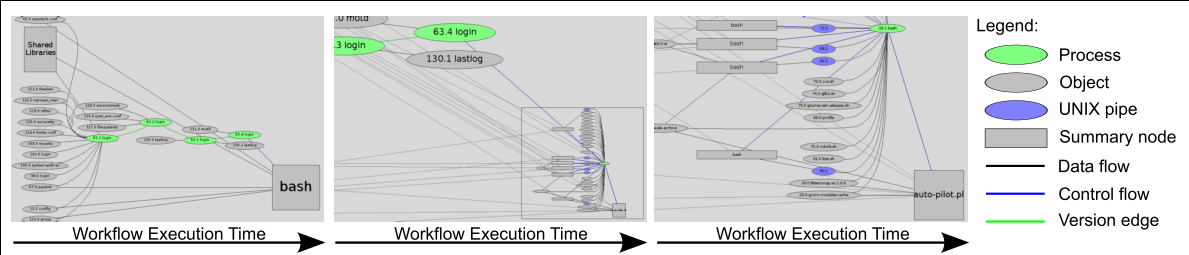
\includegraphics[width=\linewidth]{maporbiter}
	\caption{A screenshot of Mab Orbiter and its semantic zoom. Left: a high-level view of Linux’s login process and its dependencies. Middle \& Right: the progress of zooming into the bash summary node (in the lower-right corner), representing the login shell and the corresponding user session.}
	\label{fig:maporbiter}
\end{figure}

\relatedwork{Biton2007}

This paper is a demonstration that shows how user views can be used to reduce the amount of information returned by provenance queries. It allows users to select which parts of a provenance graph (referred to in this paper as a \textit{work flow}) they find relevant and have the original graph simplified to only include the parts they picked, as seen in Figure~\ref{fig:zoomuserviews}

Similar to clustering, the ZOOM interface simplifies parts of a provenance graph by collapsing nodes, however instead of creating a cluster object, ZOOM creates a replacement \textit{composite} node. The paper illustrates how it generates provenance information from logs stored on an Oracle warehouse as well as outlining some of the optimisations that can be used in Oracle 10.2 to aid in the generation of immediate provenance. The authors also discuss what properties they believe important when collapsing nodes into composites, what features make a ``good'' user view. These features include preserving the inputs and outputs from relevant nodes and hiding as much detail about irrelevant nodes as possible. In terms of size the examples in this paper are limited to graphs of 19 nodes, although extensions for larger graphs are foreseeable through extensions of the application.

This interface is similar to what I ended up designing and implementing. The primary differences are that my application uses provenance files from the PROV-N standard and that my application is designed for provenance exploration, whilst the ZOOM*UserViews system is aimed at simplifying graphs for use by other people.

\begin{figure}[h]
	\centering
	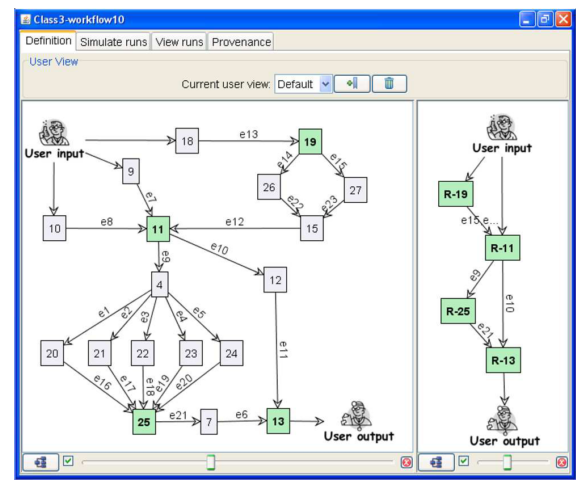
\includegraphics[width=0.8\linewidth]{zoomuserviews}
	\caption{A Screenshot of the Zoom*UserViews application. On the left is the entire provenance graph with parts selected and on the right is the simplified graph created from the selected parts.}
	\label{fig:zoomuserviews}
\end{figure}


\relatedwork{Hoekstra2014}

This paper presents an application called PRO-O-Vis that uses Sankey Diagrams in order to reflect the flow of information through activities. It discusses the application, reasoning behind representation through Sankey diagrams and a brief evaluation of their application.

This papers main contribution is an online tool that can be used to view provenance information stored in the PROV-O format. Once provenance has been uploaded it generates a viewer that allows exploration of the provenance by selecting an activity to focus on (from a dropdown menu) and presenting its related Sankey diagram. The interface is entirely web based and can be embedded in other websites completely self contained (doesn't require API calls to a server). A brief evaluation of the application has been made using four different sources and issues were found regarding input that had a large number or related activities, this could sometimes cause a delay in generating multiple Sankey diagrams. The paper briefly argues the use of Sankey diagrams over DAG graphs as they more easily allow visualisation of magnitude of flow within a network, comparatively complex DAG graphs can make it hard to view this information.

This application differs from other visualisation tools in the field as it's implemented completely in web tools whilst many of the visualizers run on Java. Because of this it is one of the easiest visualisation tools to install and get running because you mearly have to use a web browser. I used this as inspiration for implementing my prototype as a web application. 

\begin{figure}[h]
	\centering
	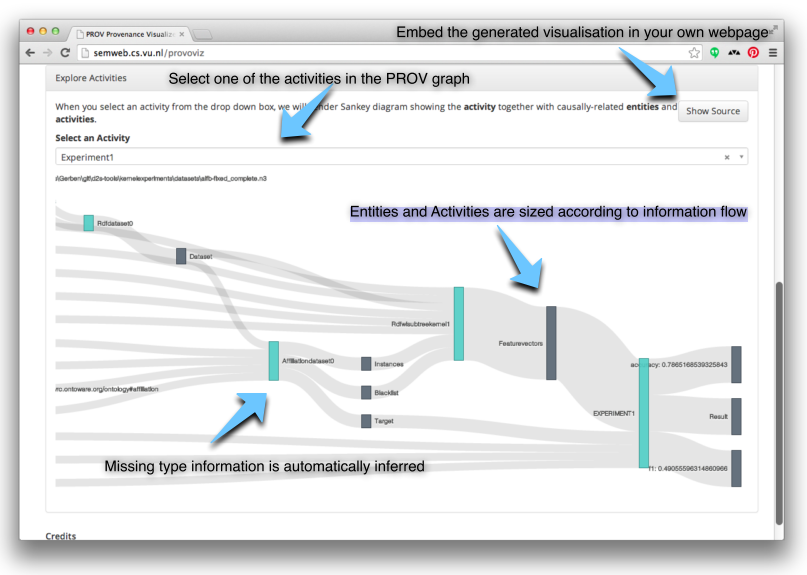
\includegraphics[width=0.8\linewidth]{provovis}
\caption{Overview report of a runtime experiment, generated by the Prov-O-Vis system.}
	\label{fig:provovis}
\end{figure}

\relatedwork{Callahan2006}

This is one of the earlier papers mentioning the concept of provenance as we know it today. Published at SIGMOD in 2006, this paper discusses the importance of provenance in generating visualizations. It presents an application called VisTrails that can be used to create visualizations whilst recording provenance during exploration to aid in later scrutiny and replication.

This paper states that existing visualization tools are limited because they do not record the provenance of their outputs. VisTrails improves on the downfalls of existing visualization tools through the use of provenance. This paper was written before any provenance standards~\cite{Macko2012} so the application instead stores all relevant provenance information in an XML formatted file. The application uses provenance in order to record \textit{evolving dataflows}, (where a dataflow is a form of visualization pipeline) allowing the modification of existing dataflows in order to compare and contrast resulting visualisations. Because provenance is captured related to changes to dataflows, it's possible at any point to check the history of a particular dataflow and identify what modifications where made to get to its current state. The VisTrails system was demonstrated through 3 examples although no references are made to any current real life uses of the application.

This paper is interesting as it's one of the earliest papers I've found in my research that identifies the importance of provenance. Its example of using provenance for visualization replication also shows how adaptable provenance can be to different scenarios, particularly its usefulness in exploratory situations. Its an important paper in order to be able to understand how the concept of provenance evolved into its current form.

\begin{figure}[h]
	\centering
	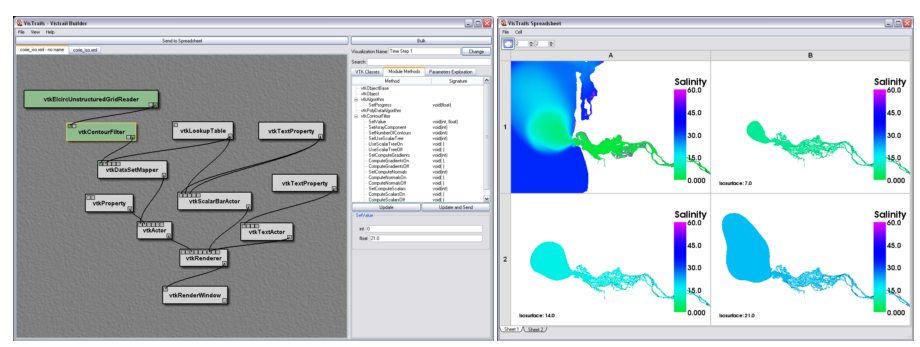
\includegraphics[width=0.9\linewidth]{vistrails}
	\caption{A screenshot of the VisTrails system. On the left you can see the provenance of a figure from a report. On the right is different versions of that figure that have been created.}
	\label{fig:vistrails}
\end{figure}

\relatedwork{Borkin2013}

This paper focuses on the visualisation of provenance information relating to filesystem: the read and writes between processes and files. The authors implement a visualization tool called InProv and both qualitatively and quantitatively compare it's effectiveness to one of the standard provenance visualisation tools Orbiter\cite{Seltzer2011}.

This papers main contributions are: Firstly, qualitative research with domain experts in order to create a set of requirements for a provenance visualiser. Secondly, InProv a provenance visualization tool that uses a radial layout and chronological clustering. Thirdly, a quantitative user study comparing the effectiveness of the two interfaces InProv and Orbiter. The qualitative research was undertaking via semi-structured one hour long interviews. They asked the domain experts to talk about how they used provenance information as well as demonstrating their daily workflows. Using results from the qualitative research they created a set of core tasks they wished to accomplish and used radial visualisation to create the InProv tool. The user study had 27 participants who where asked to accomplish tasks of varying difficulty on both the InProv and Orbiter interfaces. The metrics used to analyse performance where seconds required to complete task as well as percentage of correctly completed tasks. In most cases the difference between time to complete tasks was not significantly different between the two interfaces. However using a new clustering algorithm that clusters nodes based on time of activity (compared to process tree clustering) was shown to have significant improvement on task completion time by as much as 90 seconds.

This paper provides a lot of useful quantitative and qualitative information through its well laid out user studies. Of most interest is the interviews with domain experts. Also the choice of using \textit{time based hierarchical grouping} is of particular interest because of the large impact it had upon improving usability. This paper makes the largest attempt at conducting a usability study and my tasks were influenced by the tasks the use in this paper.

\begin{figure}[h]
	\centering
	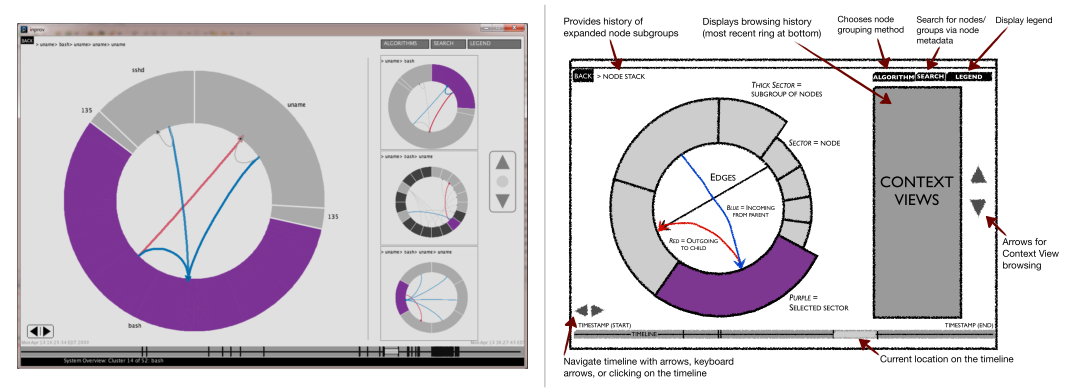
\includegraphics[width=0.8\linewidth]{filesystem}
	\caption{A screenshot and mockup of the InProv visualisation interface using radial diagrams.}
	\label{fig:filesystem}
\end{figure}
 % literature review

\chapter{Challenges}
% Some challendges of showing/controlling clustered PROV
% Automatic clustering. 
% Naming. 
% False connections.

This clustering seems promising to reduce the size, and so, the complexity, of the visible provenance graph 
%% I altered this as it sounds passive but if the user actually did the action, that is very active
in an interface.
Many challenges remain about the ways to make the clustering interface work well for users, 
so they can do clustering, and then to explore the graph. This section discusses challenges we have encountered.

\section{Specification of user-defined clusters}
\label{sub:introduction_to_clustering}

A clustering action takes a set of nodes and combines them. 
Our interface follows the established interface method to select multiple items,
hold down \textit{ctrl} then click each node, once multiple nodes are selected a contextual link will appear in the details panel (like the blue links in Fig.~\ref{fig:fitness-grouped}) allowing the user to group them. 
This works well for combining a small number of nodes. 
When the user wants to combine a larger number of nodes, 
it would be useful to add a regular language, 
so the user can define a property for all the nodes to be clustered.
For example, suppose each day's Fitbit data was a separate node.
The user may want to cluster them to a single node,
with an expression such as ``cluster all the nodes where the name is `Fitbit-*-*-Jan-2016'.'' 
The language should be able to refer to a variety of node attributes, such as Date, Source, Type, etc.

This may go beyond just features of the node, to include the relationship between this node and others: 
for example, ``cluster all Fitbit nodes that are not used in a particular report.'' 
It may be useful to support parameterised clustering, 
where one command creates multiple clusters 
(for example, ``cluster all the Fitbit nodes from each month, separately, into a month-granularity cluster'). 
It will be challenging to design such a language, so that it is both powerful and easy to learn and use.
%
Some automation may help, with where the platform suggesting clusterings, based on workloads of provenance queries recorded (for example, one might cluster nodes which are frequently accessed together).

\section{Useful naming}

Once nodes have been clustered, it is difficult to automatically generate a name 
that the user will find meaningful for the new cluster~\cite{Schaffer1996, Abello2006}. 
Automating this process requires domain knowledge and it may also need deep models of the user and their needs.
This would be a substantial undertaking. 
For example, it may demand recognition that \textit{vim}, \textit{emacs} and \textit{nano} are all text editors? 
In an early version of our prototype, a new cluster-node was given a short random alpha-numeric name. 
However, this made the graph incomprehensible, with users needing to manually update the name immediately
so that they could understand the graph. 
Our current, still simple approach uses the name of the node in the cluster with the shortest distance from the root with the text ``group'' appended to the end. 
So, for example, in the transition from Figure~\ref{fig:fitness-ungrouped} to Figure~\ref{fig:fitness-grouped}, the node created would be named \textit{Fitness-Summary group}.


\section{Avoiding false dependencies}

Clustering is a simple type of graph rewriting, which creates an abstraction of the graph and in turn simplifies details of the original graph. This can produce false dependencies: these are newly implied lines of lineage, created by the clustering, and they falsely suggest that one entity had influence upon another. 
Worse yet, circular dependencies may occur, along with other violations of the constraints defined in the PROV-CONSTRAINT W3C document~\cite{w3c-prov-constraints}. For example, if the clustering set in the example of Fig.~\ref{fig:fitness-ungrouped} only included nodes \{\texttt{fitness-summary}, \texttt{CalorieIntakeFeed}\},  then a simple replacement of these nodes with a node $x$ would result in a circular dependency, namely $\langle x \; \mathtt{wasGeneratedBy} \; \mathtt{summarize}\rangle$ and $\langle \texttt{summarize} \; \texttt{used} \; x \rangle$, you can see this in Fig.~\ref{fig:loop}.
A theoretical formulation of provenance abstraction by \textit{grouping} (clustering) has been proposed in~\cite{Missier2014} to describe this and other problems that occur with clustering, along with simple algorithms for grouping arbitrary sets of nodes. 
Essentially, that work showed that to avoid false dependencies, as well as circular data dependencies, one must first compute a \textit{closure} operation that extends the user-selected nodes with all other nodes that sit on any path amongst these initial clustering nodes.
Combining this prior work with our user-oriented provenance navigation model can lead to a provably correct clustering mechanism. 
%A check could be made comparing suggested lineage of nodes around a cluster selecteion before and after a clustered node is created to see if any false connections exits. In some cases false connections may be desireable to obviscate sensitive information.

\begin{figure}[h]
	\centering
	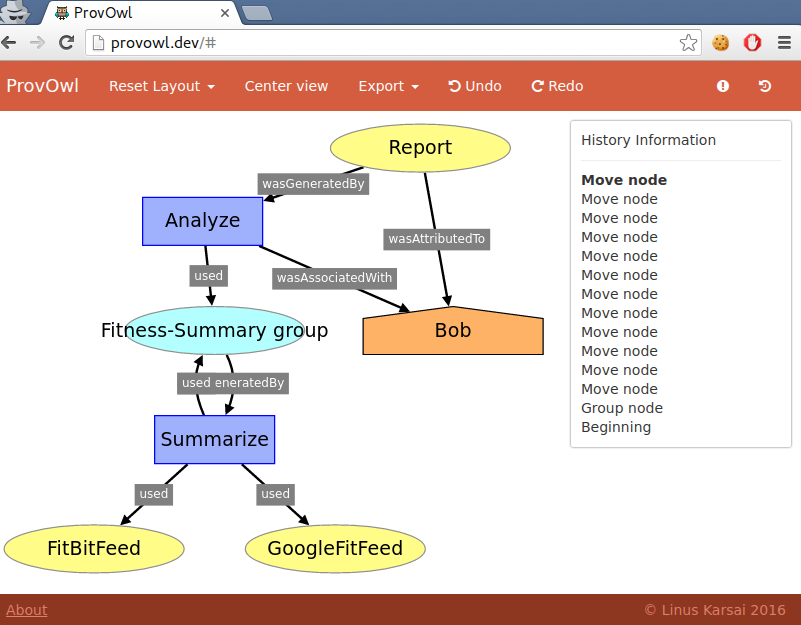
\includegraphics[width=\linewidth]{loop}
	\caption{When grouping on \{\texttt{fitness-summary}, \texttt{CalorieIntakeFeed}\} a circular dependency is caused between \texttt{Fitness-Summary group} and \texttt{Summarize}. The panel on the right can be toggled by the history button above and shows a list of user actions with the current state indicated in bold. Users can use the \textit{Undo} and \textit{Redo} buttons to move between actions.}
	\label{fig:loop}
\end{figure}


 % challenges of clustering

\chapter{Initial interface}
\label{cha:initial_interface}
% Initial interface ideas, with a couple of screenshots, and a paragraph about implementation

Our interface reads provenance data stored in the PROV format~\cite{primer2013} and renders a directed acyclic graph that users can explore by zooming, panning, rearranging nodes and grouping nodes manually. 

%% IN UI work, accessible has special meaning
We implemented this as a web application. We use the Cytoscape.js\footnote{Cytoscape.js: Graph theory library for analysis and visualisation \url{http://js.cytoscape.org/}} because it has good support for graph theory. 
Files are loaded completely client-side, to reduce bandwidth. If faster analysis were required, it may require use of a combination of server-side and client-side processing.

%We implemented this interface as a web application because we had the highest level of expertise in web debelopment and it is a platform that is easily accessible by users. The standard technology for data visualisation in a browser is the D3.js\footnote{D3: Data Driven Documents \url{https://d3js.org/}} JavaScript library, however this interface is implemented using the Cytoscape.js\footnote{Cytoscape.js: Graph theory library for analysis and visualisation \url{http://js.cytoscape.org/}} because it specifically focuses on graph theory. Files are loaded completely client side in order to reduce bandwidth. If high powered analysis of provenance was required it may later be necessary to have server side processing in conjunction to client side processing. 

\section{Features}

This section explains how the design of our interface fulfils the seven visualisation tasks outlined by Ben Shneiderman~\cite{Shneiderman1996}: \textit{overview}, \textit{zoom}, \textit{filter}, \textit{details-on-demand}, \textit{relate}, \textit{history}, \textit{extract}. 

\subsection{Movement and Rearranging}
On first opening a provenance graph, the viewport is positioned to fit the entire graph on screen. This gives users an overview of the provenance. Users can then move the viewport around by clicking and dragging. Zooming is accomplished by using the scroll wheel. 

By default the graph's overall layout is determined using the JavaScript library dagre\footnote{Dagre: supports lay out of directed graphs client-side. The main skeleton of algorithm comes from ``A Technique for Drawing Directed Graphs''~\cite{Gansner1993}}, with other layout options, such as circle and breadth-first, available using the ``Reset Layout'' menu (visible on the top bar, second from the left in the figures). Users can also re-arrange nodes as they wish by clicking and dragging on a node. 

\subsection{Details-on-demand}
Selecting a node shows the details panel, as in Fig.~\ref{fig:fitness-grouped}. This displays other information about the node and contextual functions such as renaming nodes (the blue link at the bottom of the panel) or grouping nodes.

\subsection{Grouping}

Users can select multiple nodes at once, by clicking on each whilst holding down \textit{ctrl}. 
Once multiple nodes have been selected, the information panel will contain a link to group the nodes. 
Selecting this moves the nodes together, replacing them with a single composite node, represented by a light blue oval, 
with default name based on the name of the node closest to the root plus the word ``group''. 

\subsection{History}

%A vital task in exploration interfaces is that of history~\cite{Shneiderman1996}. 
Having the ability to undo and redo 
actions is critical to ensure that users can confidently and safely explore the information, 
without fear of causing permanent damage~\cite{Shneiderman1996}. 
Our interface tracks the movement and grouping of nodes. 
Then undo and redo buttons allow users to step through through these actions. 
A history pane can be toggled, by clicking the top right history icon (this pane is visible on the right of Fig.~\ref{fig:loop}), to show what current step of history a user is at.

\subsection{Sharing}

The ``Export'' menu item (in the top bar of the figures)
saves an image of the current graph with all the user modifications. 
This can either save the entire graph or be limited to the current viewport,
if the user wanted to focus on a certain section.
 % explanation of interface

\chapter{Implementation}

\section{Web Technologies}
\label{sec:web_technologies}

As we saw above, I implemented my prototype as a web application. The criteria for picking an implementation platform was that of accessibility to users and speed of development. Using that criteria I decided to make my prototype a web application as it's only entry barrier to users is that of a modern web browser. Web applications are a field that I have experience with and can quickly develop in. 

There are a few pitfalls to this approach that can be addressed through alternative implementations. Because my application is primarily a prototype for illustrating effective exploration features, the issue of scale is not one that was addressed. If a web application was used for enterprise size provenance files the application may soon run out of resources required to render it.

An alternative to a web application would be to write the prototye in an OS independent language such as Java or Python; this would allow wide accessibility and more fine grained control of machine resources. However if an OS level language was chosen issues could later occur in presenting provenance on mobile devices as there aren't may languages that run on both desktop and mobile devices without heavy modifications. Consequently if an OS dependant languages such as Apple's swift of Microsoft's C\# was used features and code would have to be replicated for the different OS languages (assuming that OS independent accessibility is an important criteria).

The standard technology for data visualisation in a browser is the D3.js\footnote{D3: Data Driven Documents \url{https://d3js.org/}} JavaScript library. However as mentioned earlier, I used Cytoscape.js to implement my interface because it's specifically focused on graph theory and has a lot of inbuilt functions such as rendering and events. If this application was to be re-written using D3, a lot more of the fundemental functions of Cytoscape would have to be written from scratch, however it would allow for more fine-grained control of the appplication, this could particularly be useful when dealing with exceptionally large files.

\section{Client Side Processing}
\label{sec:client_side_processing}

As we saw before, the visualiser loads the file on the client side and renders it locally. When first outlining features of the application I wanted it to be primarily stand alone. This means that even though it can run of a web server, you could just as easily run it locally on your computer with minimal effort because all proccessing and computation is done client side. 

However server side computation may be a useful feature for the future, a server with higher computational power and resources may be able to find and analyze interesting details about the file. The naive approach to accomplishing this would to have the file uploaded to the server, analytics run on the provenance and then results downloaded back to the client. An alternative approach however would to have the client select only the neccessary sectinos required for analysis and send those to the server. The client could then render the provenance locally whilst results where computed and finally render the results onto the already drawn graph. This allows the user to begin exploring the graph immediately as well as minimising the amount of bandwidth used by the application.

\section{Node Clustering}
One of the earliest features we discussed when outlining how to visualise provenance was the ability to cluster and create composite nodes. The feature of allowing multiple nodes to be grouped into a single representative node has two main purposes. Firstly it allows simplification of the graph, this is useful when showing someone a speficit section of the graph as well as easier conceptual understanding when exploring. Secondly it is useful when securing graphs and composite nodes can be used to obviscate information.

Cytoscape.js doesn't have a group feature, so it was required to write one from scratch. The key test for this function is that grouping and ungrouping nodes is undestructive: if a series of nodes are grouped and then ungrouped the resulting graph must be isomorphic to the original.

\begin{figure}[h]
  \centering
  \begin{subfigure}[t]{0.5\textwidth}
    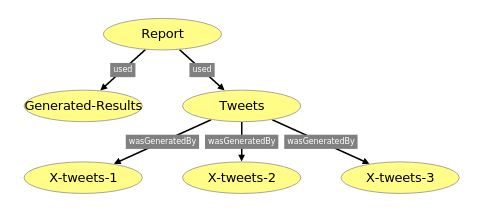
\includegraphics[width=\textwidth]{ungrouped}
    \caption{Graph with no composite nodes}
  \end{subfigure}
  ~
  \begin{subfigure}[t]{0.5\textwidth}
    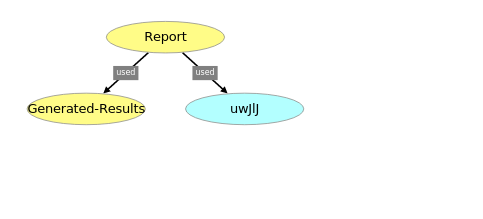
\includegraphics[width=\textwidth]{grouped}
    \caption{Same graph with a composite node}
  \end{subfigure}
  \caption{An example of a composite node containing the \textit{Tweets}, \textit{X-tweets-1}, \textit{X-tweets-2} and \textit{X-tweets-3} nodes.}
\end{figure}

Nodes removed from Cytoscape.js can be `restored' into their original position, unfortunately any edged associated with the node are permenately destroyed. It is neccessary then to store the edges as a data field in the composite node so that when restoring nodes, edges can also be recreated. 

\begin{figure}[h]
  \centering
  \begin{lstlisting}
 // Create composite node and fields for original edges and nodes.
 Create new CompositeNode 
 CompositeNode.originalEdges = All edges in neighbourhood of selected nodes
 CompositeNode.originalNodes = All nodes that where grouped

 // Create new edges from external nodes to CompositeNode
 for each edge in neighbourhood {
  if (edge != internal to group)  {
    Create new Edge({from: externalNode, to:compositeNode})
  }
 }

 // Remove original nodes
 Remove selected nodes
 \end{lstlisting}
 \caption{Pseudocode: Creaing a composite node}
\end{figure}

However the above code only works in a limited scenario: ungrouping nodes in the oposite order of creation. For example if you created comisite nodes $A$, $B$, $C$ (cronologically and all with neighbouring edges) you would have to ungroup them in the following order: $C$, $B$, $A$. If you where to for example ungroup node $A$ first, when ungrouping $C$ it would try to restore edges to the now non-existent $A$ compsosite node. In order to tackle this I created the group manager class.

The Group Manager class is the primary way of keeping track of nodes that are hidden inside composite nodes. It contains a tree data structure that references all the groups as well as their child nodes/groups. Now when ungrouping nodes this class is called and the parent group of the child node requested, then a new temporary edge is created to the composite node and the original edge stored in a \textit{hanging edges} object until it can be restored. Every time a group is created or destroyed the \textit{hanging edges} object is queried to see if any originl edges can be recreated.

\subsection{Clustering example: Without \textit{Group Manager} or \textit{Hanging Edges}}

Below is an example of issues that occur when trying to ungroup nodes in the incorrect order without the supporting classes \textit{Group Manager} and the hanging edges object. As seen in the final step, all the edges are lost, a less than ideal situation and in failure of the primary test of having an isomorphic graph after grouping and ungrouping nodes.

\begin{figure}[H]

  \begin{subfigure}[t]{0.5\textwidth}
    \centering
    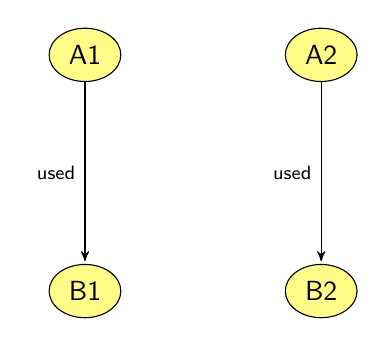
\begin{tikzpicture}
      \node[main node] (A1) {A1};
      \node[main node] (A2) [right of=A1] {A2};
      \node[main node] (B1) [below of=A1] {B1};
      \node[main node] (B2) [below of=A2] {B2};
      \path (A1) edge node[left] {used} (B1);
      \path (A2) edge node[left] {used} (B2);
    \end{tikzpicture}
    \caption{Nodes $A1$ and $B1$ are linked, nodes $A2$ and $B2$ are linked.}
  \end{subfigure}
  ~
  \begin{subfigure}[t]{0.5\textwidth}
    \centering
    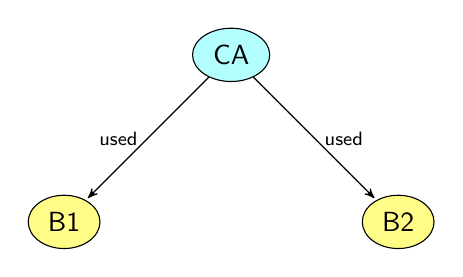
\begin{tikzpicture}
      \node[main node, group] (CA) {CA};
      \node[main node] (B1) [below left of=CA] {B1};
      \node[main node] (B2) [below right of=CA] {B2};
      \path (CA) edge node[left] {used} (B1);
      \path (CA) edge node[right] {used} (B2);
    \end{tikzpicture}
    \caption{Group nodes $A1$ and $A2$ into composite node $CA$. Stored inside the composite node is the original edges from $A1\rightarrow B1$ and $A2\rightarrow B2$.}
  \end{subfigure}
  \begin{subfigure}[t]{0.5\textwidth}
    \centering
    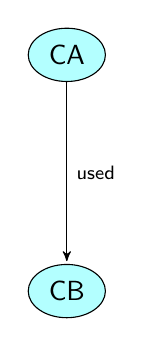
\begin{tikzpicture}
      \node[main node, group] (CA) {CA};
      \node[main node, group] (CB) [below of=CA] {CB};
      \path (CA) edge node[right] {used} (CB);
    \end{tikzpicture}
    \caption{Group nodes $B1$ and $B2$ insto composite nodes $CB$. Stored inside the composite node $CB$ is the edges from $CA\rightarrow B1$ and $CA\rightarrow B2$.}
  \end{subfigure}
  ~
  \begin{subfigure}[t]{0.5\textwidth}
    \centering
    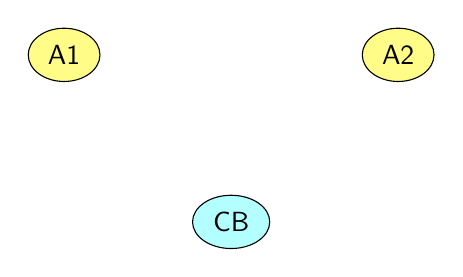
\begin{tikzpicture}
      \node[main node, group] (CB) {CB};
      \node[main node] (A1) [above left of=CB] {A1};
      \node[main node] (A2) [above right of=CB] {A2};
    \end{tikzpicture}
    \caption{Ungroup $CA$. It will try to create adges between $A1\rightarrow B1$ and $A2\rightarrow B2$, because $B1$ and $B2$ are currently in a group, the new edges will fail and not be rendered.}
  \end{subfigure}
  \begin{subfigure}[t]{0.5\textwidth}
    \centering
    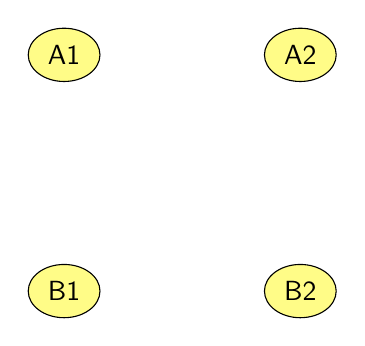
\begin{tikzpicture}
      \node[main node] (A1) {A1};
      \node[main node] (A2) [right of=A1] {A2};
      \node[main node] (B1) [below of=A1] {B1};
      \node[main node] (B2) [below of=A2] {B2};
    \end{tikzpicture}
    \caption{Ungroup $CB$. Edges between $CA\rightarrow B1$ and $CA\rightarrow B2$ will try to be restored but because there's no $CA$ in the graph these will fail.}
  \end{subfigure}
\end{figure}

\subsection{Clustering example: Working isomorphic grouping with helping classes.}
As mentioned previously we want to complete the test of having an isomorphic graph after grouping and ungrouping nodes. To do this we use both a class \textit{GroupManager} and an array \textit{HangingEdges}. The \textit{GroupManager} stores a tree to monitor groups and nodes inside them, it also has some helper functions for adding groups and finding the upmost group of a certain node. The \textit{HangingEdges} array is simply a list of edges that couldn't be restored because one or more of the connected nodes where missing.

In the figure below the left hand side shows the state of the graph, whilst the right hand side shows the \textit{GroupManager} as well as the content of \textit{HangingEdges}.

\begin{figure}[H]

  \begin{subfigure}[t]{0.5\textwidth}
    \centering
    \renewcommand\thesubfigure{A1}
    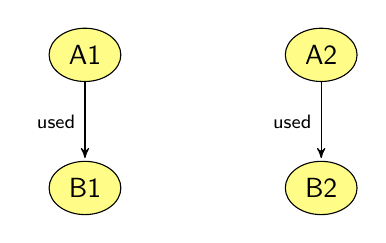
\begin{tikzpicture}
      \node[main node] (A1) {A1};
      \node[main node] (A2) [right of=A1] {A2};
      \node[main node] (B1) [below = 1cm of A1] {B1};
      \node[main node] (B2) [below = 1cm of A2] {B2};
      \path (A1) edge node[left] {used} (B1);
      \path (A2) edge node[left] {used} (B2);
    \end{tikzpicture}
    \caption{Nodes $A1$ and $B1$ are linked, nodes $A2$ and $B2$ are linked.}
  \end{subfigure}
  ~
  \begin{subfigure}[t]{0.5\textwidth}
    \renewcommand\thesubfigure{A2}
    \centering
    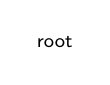
\begin{tikzpicture}
      \node[] (root) {root};
    \end{tikzpicture}
    \caption{The GMTree (Group Manager Tree) is currently empty and Hangingedges = [].}
  \end{subfigure}
  \begin{subfigure}[t]{0.5\textwidth}
    \centering
    \renewcommand\thesubfigure{B1}
    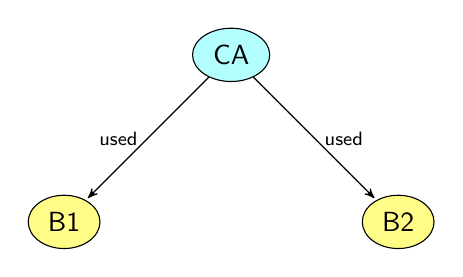
\begin{tikzpicture}
      \node[main node, group] (CA) {CA};
      \node[main node] (B1) [below left of=CA] {B1};
      \node[main node] (B2) [below right of=CA] {B2};
      \path (CA) edge node[left] {used} (B1);
      \path (CA) edge node[right] {used} (B2);
    \end{tikzpicture}
    \caption{Group nodes $A1$ and $A2$ into composite node $CA$. Stored inside the composite node is the original edges from $A1\rightarrow B1$ and $A2\rightarrow B2$.}
  \end{subfigure}
  ~
  \begin{subfigure}[t]{0.5\textwidth}
    \centering
    \renewcommand\thesubfigure{B2}
    \begin{tikzpicture}
      \node[] (root) {root};
      \node[below = 1cm of root] (CA) {CA};
      \node[below right = 1cm of CA] (A1) {A1};
      \node[below left = 1cm of CA] (A2) {A2};
      \path (root) edge (CA);
      \path (CA) edge (A1);
      \path (CA) edge (A2);
    \end{tikzpicture}
    \caption{The GMTree holds information about $CA$, $A1$ and $A2$. Hangingedges = [].}
  \end{subfigure}

  \begin{subfigure}[t]{0.5\textwidth}
    \renewcommand\thesubfigure{C1}
    \centering
    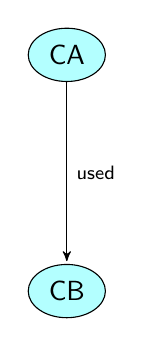
\begin{tikzpicture}
      \node[main node, group] (CA) {CA};
      \node[main node, group] (CB) [below of=CA] {CB};
      \path (CA) edge node[right] {used} (CB);
    \end{tikzpicture}
    \caption{Group nodes $B1$ and $B2$ insto composite nodes $CB$. Stored inside the composite node $CB$ is the edges from $CA\rightarrow B1$ and $CA\rightarrow B2$.}
  \end{subfigure}
  ~
  \begin{subfigure}[t]{0.5\textwidth}
    \centering
    \renewcommand\thesubfigure{C2}
    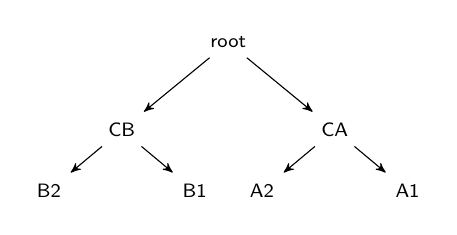
\begin{tikzpicture}
      \node[] (root) {root};
      \node[below right = 1cm of root] (CA) {CA};
      \node[below right = 0.5cm of CA] (A1) {A1};
      \node[below left = 0.5cm of CA] (A2) {A2};

      \node[below left = 1cm of root] (CB) {CB};
      \node[below right = 0.5cm of CB] (B1) {B1};
      \node[below left = 0.5cm of CB] (B2) {B2};
      \path (root) edge (CA);
      \path (CA) edge (A1);
      \path (CA) edge (A2);
      \path (root) edge (CB);
      \path (CB) edge (B1);
      \path (CB) edge (B2);
    \end{tikzpicture}
    \caption{The GMTree holds information about all nodes. Hangingedges = [].}
  \end{subfigure}

  \begin{subfigure}[t]{0.5\textwidth}
    \centering
    \renewcommand\thesubfigure{D1}
    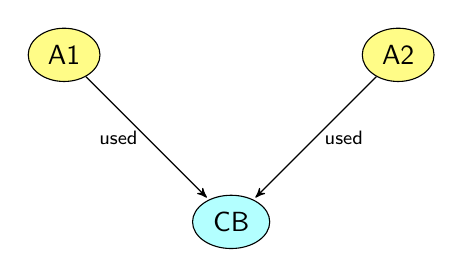
\begin{tikzpicture}
      \node[main node, group] (CB) {CB};
      \node[main node] (A1) [above left of=CB] {A1};
      \node[main node] (A2) [above right of=CB] {A2};
      \path (A1) edge node[left] {used} (CB);
      \path (A2) edge node[right] {used} (CB);
    \end{tikzpicture}
    \caption{CA is ungrouped and removed from the group manager tree. The original edges $A1\rightarrow B1$ and $A2\rightarrow B2$ can't be restored because B1 and B2 are currently hidden inside CB, these edges are stored in the hanging edges object. New edges are created by finding the upmost node using the group manager tree.}
  \end{subfigure}
  ~
  \begin{subfigure}[t]{0.5\textwidth}
    \centering
    \renewcommand\thesubfigure{D2}
    \begin{tikzpicture}
      \node[] (root) {root};
      \node[below = 1cm of root] (CB) {CB};
      \node[below right = 0.5cm of CB] (B1) {B1};
      \node[below left = 0.5cm of CB] (B2) {B2};
      \path (root) edge (CB);
      \path (CB) edge (B1);
      \path (CB) edge (B2);
    \end{tikzpicture}
    \caption{The GMTree holds information about $B$ nodes. $A$ nodes have been remove because they've been ungrouped. Hangingedges = [$A1\rightarrow B1$, $A2\rightarrow B2$].}
  \end{subfigure}

  \begin{subfigure}[t]{0.5\textwidth}
    \centering
    \renewcommand\thesubfigure{E1}
    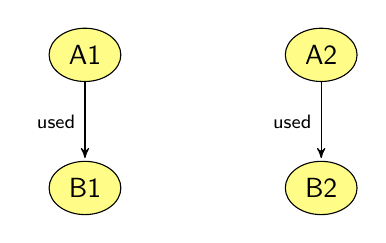
\begin{tikzpicture}
      \node[main node] (A1) {A1};
      \node[main node] (A2) [right of = A1] {A2};
      \node[main node] (B1) [below = 1cm of A1] {B1};
      \node[main node] (B2) [below = 1cm of A2] {B2};
      \path (A1) edge node[left] {used} (B1);
      \path (A2) edge node[left] {used} (B2);
    \end{tikzpicture}
    \caption{CB is ungrouped and removed from the group manager tree. An attempt to restore hanging edges is made and both $A1\rightarrow B1$ and $A2\rightarrow B2$ are restored.}
  \end{subfigure}
  ~
  \begin{subfigure}[t]{0.5\textwidth}
    \centering
    \renewcommand\thesubfigure{E2}
    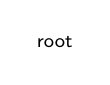
\begin{tikzpicture}
      \node[] (root) {root};
    \end{tikzpicture}
    \caption{The GMTree is empty because there's no groups. Hangingedges = [] because the previously stored edges have been restored.}
  \end{subfigure}
\end{figure}
 % technical implementation decisions

\chapter{Usability study design}

Provenance graphs can be quite large. They also hold and present information in a variety of aspects: \textit{nodes}, \textit{relationships} and \textit{attributes}. Node data is the graph information related to a nodes: the name of a node as well as its type (eg. entity, agent). Relationship data is information implied through connections; an edge between two nodes represents some sort of relationship between them, whether it be that one \textit{used} the other or that an entity was generated by another node. Attribute data is the properties given to a node, usually generated during collection. For example, a node representing a stream of twitter data may have a start and end property specify the times that the feed covers\footnote{Because provenance presents data in three different aspects (nodes, relationships and attributes), It becomes difficult to secure because a security model would have to take into account the three different types of data\cite{Braun2008}}.

Because of this large and heterogeneous amount of information stored in provenance graphs I found it important that an interface allowed users to interactively explore the graph rather than just using static images of provenance graphs. It is because of this that I decided to undertake my usability study using a prototype interface that allows clustering of nodes. 

\section{Interview format}
\label{sec:interview_format}

Interviews were undertaked with participants in order to guage how effective clustering is as a form of graph simplification and a tool for representing information. The participants were asked to complete a series of expercises using the ProvOwl interface whilst I took notes. They undertook these exercises on my laptop with the browser in full-screen mode in order to limit distractions. A mouse was provided in case users hadn't used a MacBook trackpad before. The interviews were undertaken wherever was most convenient to the participant, this included at my desk, participant's houses or coffee shops.

The study was split into four sections: background information, provenance primer, three exercises and a SUS questionnaire. 

\subsection{Background Information}
\label{sec:background_information}

General background information was collected about each participant. Gender, age groups as well as highest level of education. These were recorded in order to identify any demographic skew that I may have in my cohort as well as in case any unexpected correlations occurred. As a last general question I also asked if they had heard of the term \textit{provenance} before, and if so to explain what it meant. Because provenance is used in other fields (such as accounting and art dealership) I wanted to identify anyone who had previous concepts of provenance and lineage to identify if this effected their ability to interpret provenance graphs.

\subsection{Provenance Primer}
\label{sec:provenance_primer}

After the participant had answered the general background questions they were given a information sheet explaining the concept of provenance in breif and showing an example of a provenance graph as well as explanations of what the different coloured and shaped nodes meant (\ref{prov-primer}). This allowed participants to have a uniform understanding of the concept of provenance reguardless of whether they had heard of it before or not. Notes were taken of any questions the participant had whilst reading the information sheet.

\subsection{Exercises}
\label{sec:exercises}

\begin{figure}[b]
\caption{Scenario for exercise one. View text in context in Appendix TODO}
\begin{framed}
\begin{flushleft}
Suppose you are Alice. You have been using your FitBit and Withings scales for 3 years to reduce your weight to 61kg and to increase your physical activity to 8000 steps a day. You have just linked your FitBit account to two friends, Bob and Carol. Recently FitBit introduced a fitness score that is shared and ranked with your friends\textellipsis This makes you wonder just how your score has been calculated.
\end{flushleft}
\end{framed}
\end{figure}
\begin{figure}[b]
\caption{Scenario for exercise two. View text in context in Appendix TODO}
\begin{framed}
\begin{flushleft}
You are a researcher creating a citizen-data-report that recommends strategies for improving the fitness of your local community. You have step, location, weight and calorie information about members of the community. You are using this information to create multiple reports regarding fitness and weight information which will be used to support a final report addressed to the community on strategies that can be used to improve overall fitness. 
\end{flushleft}
\end{framed}
\end{figure}
\begin{figure}[b]
\caption{Scenario for exercise three. View text in context in Appendix TODO}
\begin{framed}
\begin{flushleft}
This provenance graph is an abstract representation of a report based on twitter data. 
\end{flushleft}
\end{framed}
\end{figure}

Overall there was three exercises. Each exercise described a particular scenario assosiated with a provenance file and required users to answer questions and complete tasks related to that provenance file. 

For example, in the first exercise the user is asked to imagine that they're Alice, they track their fitness information with a Fitbit for steps and a Withings scale for weight (you can find the exact example in \ref{interview-questionnaire}). The first question of each exercise was a simple identification query. The participant would be asked to identify different aspects of the graph or to trace the lineage from a certain element. This allowed the participants to take their time when first analysing the graph as well as giving me an understanding of their mental model.

Each exercise was progressively more conceptually difficult than the previous. The first, as mentioned before, invovled putting yourself in the shoes of Alice and answering a series of questions related to your data. The provenance graph they are given to explore starts with nodes detailing their weight and steps clustered respectively. This meant that users were required to ungroup the nodes either by clicking the ungroup button from a menu or double clicking on nodes (most users identified that double clicking would un-cluster nodes without prompting) in order to correctly answer the questions. This first exercise was completely exploration based and no modifications of the graph where required.

The second exercise invovled a larger amount of data and asked participants to imagine themselves as the curator of a citizen science project. Data was been tracked about multiple users and then used in a report that gave feedback on how to improve the cohorts overall fitness. Similar to exercise one there was first a task asking the user to describe the contents of the graph to me. Following from there was two tasks that required the user cluster nodes in order to hide information. Because un-clustering was required to complete the first task users where accustomed to the concept of clustering nodes by the time they got to this task.


The third and final exercise expanded on the previous by requiring users to convey information by modifying the graph. This is silghtly different to exercise two which required the participant to \textit{hide} information, instead users had to convey a certain point through a graph. Same as above the first task asked the user to describe the graph, a bit more difficult as the graph was abstract compared to the previous two. The following two tasks where of the following format: \textit{You want to modify the graph in order to convey the following information: <information to convey>}. 

\subsection{SUS Questionnaire}
\label{sec:sus_questionnaire}

% TODO: Insert references

In order to test the effectiveness of a feature of an interface I thought it was important also to gauge how effective the interface was on a whole. The System Usability Scale has been around since 1986. It provides a quick easy way of identifying if an interface is easy to use or not. 

The SUS questionnaire consists of 10 questions each requiring a checkbox response on a scale of 1-5 stating if they strongly agree of strongly disagree. Users are asked to reply with what they intuitively feel rather than thinking about the questions for an extended period. 

\section{Coded questions}
\label{sec:coded_questions}

Each question was given a set of points, user actions that could be checked off if a user did them. For example, in question one of exercise one, the participant was asked \textit{What infroation is used to calculate your [fitness] score?}. One of the points for this question was \textit{ungrouped nodes}, so if the user ungrouped nodes while answering the question this point was ticked off. Whilst hand written notes were also taken during interviews, these checkboxes made for an easy way of identitying what common actions users undertook to complete exercises. 

Each point was assigned a code identifying what class of activity it belonged to. In the above example the ungrouping point had the code \textit{grouping-ungroup} because it's completing a grouping function and in particular an ungrouping function. 

Each of the codes are listed in Table~\ref{tab:question-codes} with an explanation of the user behaviour they map to.

\begin{table}[h]
	\centering
	\caption{List of question codes and descriptions of each.}
		\def\arraystretch{1.5}
	\label{tab:question-codes}
	\begin{tabu} to \textwidth { | l | X[l] | }
		\hline
		\textbf{Code}& \textbf{Description}  \\	
		\hline
		\hline
		grouping & Activities that involved users grouping or ungrouping nodes (by any means)\\
		\hline
		grouping-group &  When a user grouped a node \\
		grouping-ungroup & When a user ungrouped a node \\
		grouping-complex & When a user grouped a complex set of noes \\
		\hline
		\hline
		graph & Activities related to understanding a graph conceptually \\
		\hline
		graph-explain & Notice and comment on information in the graph. An example is in exercise one where some users noticed that weight data is both manually and automatically logged. This information is not usually relevant to the question. \\
		graph-understanding & Correctly understand a concept from the graph, usually directly in response to a question. \\
		\hline
		\hline
		lineage & Correctly identifying information related to the lienage of a node. \\
		\hline
		lineage-identify & Correctly identified simple lineage. \\
		lineage-implied & Correctly identified lineage passing through multiple entities. \\
		lineage-complex & Correctly identified lineage that was complex, usually identifying multiple nodes. \\
		\hline
		\hline
		interface & When a user uses a specific bit of the ProvOwl interface. \\
		\hline
		interface-export-image & Using the export -> image menu item to save an image of a graph.\\
		interface-os-screenshot & Using the operating system screenshot functionality to save an image of a graph. \\
		interface-rename & Using the rename function (found in the contexual links in a nodes details) to rename a node. \\
		interface-manual-group & Manually group nodes by ctrl+clicking multiple nodes and selecting \textit{group nodes} from the contexual menu. \\
		interface-search-group & Grouping nodes by searching for the nodes they want to use using the search function and then grouping them. \\
		\hline
		\hline
		privacy & Whether a user was privacy concious at all in relation to personal data. \\
		\hline
 
	\end{tabu}
\end{table}


 % plan of question coding etc.

\chapter{Results} % results

\chapter{Conclusions and Discussion} % discussion

\chapter{Future Work}
The prototype source code is available on GitHub\footnote{\url{https://github.com/karsai5/ProvOwl}}. The interface is also available online where you can test it with a sample graph\footnote{\url{http://provowl.com/?file=/prov-examples/provn/threenode.provn}}.
We describe features under development to improve usability.

We propose to create a regular expression language to select nodes, as mentioned in the section on challenges. 
This will enable users to select nodes in cases such as:
(i) Select all nodes with the name ``*Feed''
(ii) Select all nodes \textit{not} influencing the ``Summarize'' node
(iii) Select all children of ``Fitness-Summary''.
For large graphs, this could allow for faster user-directed simplification of a graph. 

As an extension of this, the language should describe parametered clustering, so users ask for multiple similar clusters to be formed. For example ``Create clusters from nodes the same depth from the root'' or even using data inside the nodes ``Create clusters from nodes that have the same creation date''.  

This could also impact the way nodes are automatically named. If the user created clusters from nodes that all have the same creation date, the system may infer that the name for the new node should include the creation date.

We also wish to extend the PROV standard to include descriptions of cluster nodes. This would allow a user to cluster nodes manually, export the PROV file with cluster descriptions and then share with someone else. This \textit{extraction}, being able to export your current state of exploration, would allow further exploration from the current state later on or even sharing with other users for further analysis.
 % planned future work

\printbibliography

\newcommand{\multipdf}[3][]{
	\label{sec:#2}
	\includepdf[pages=1,frame=true,width=\linewidth,pagecommand=\section{#2}]{#3}
	\includepdf[pages=2-#1,frame=true,width=\linewidth]{#3}
}

\newcommand{\singlepdf}[2]{
	\includepdf[pages=1,frame=true,width=\linewidth,pagecommand=\section{#1}]{#2}
}

\begin{appendices}
	\renewcommand{\thesection}{\appendixname~\Alph{section}}

	\singlepdf{Provenance Primer}{pdfs/provenance-primer.pdf}

	\multipdf{Interview Questionnaire}{pdfs/questionnaire.pdf}

	\section{PROV File: IR-Baseline}
	\label{sec:prov_file_ir_baseline}
	
	\lstinputlisting[style=provn]{provn/IR-baseline.provn}

\end{appendices}



\end{document}
